% 02.tex
% Benjamin Davies
% 2017 03 03

\begin{enumerate}

	\item
	Recall that a function~$f(x)$ has a \emph{stationary} point at~$x^*$ if~$f'(x^*)=0$.
	Find the stationary points of the following functions.
	%
	\begin{enumerate}

		\item
		$a(x)=(x-1)^2$.
		%
		\begin{solution}
			Differentiating~$a(x)$ with respect to~$x$ gives
			\[ a'(x)=2(x-1). \]
			The equation~$a'(x^*)=0$ has a unique solution~$x^*=1$.
			Hence~$a(x)$ has a stationary point at~$x^*=1$.
		\end{solution}

		\item
		$b(x)=x^2/(1-x^2)$.
		%
		\begin{solution}
			Differentiating~$b(x)$ with respect to~$x$ gives
			\[ b'(x)=\frac{2x}{(1-x^2)^2}. \]
			The equation~$b'(x^*)=0$ has unique solution~$x^*=0$.
			Hence~$b(x)$ has a stationary point at~$x^*=0$.
		\end{solution}

		\item
		$c(x)=x(x^2-3)$.
		%
		\begin{solution}
			Differeniating~$c(x)$ with respect to~$x$ gives
			%
			\begin{align}
				c'(x)
				&= x^2-3+x(2x)\\
				&= 3x^2-3.
			\end{align}
			%
			The equation~$c'(x^*)=0$ has a two solutions~$x^*=\pm1$.
			Hence~$c(x)$ has stationary points at~$x^*=\pm1$.
		\end{solution}

	\end{enumerate}

	\item
	Let~$f(x)$ and~$g(x)$ be arbitrary functions with~$x\in\R$, and let
	\[ h(x)=\frac{f(x)}{g(x)}. \]
	Apply the product rule to~$f(x)=g(x)h(x)$ to show that
	\[ h'(x)=\frac{f'(x)g(x)-f(x)g'(x)}{[g(x)]^2}. \]
	%
	\begin{solution}
		Applying the product rule to~$f(x)=g(x)h(x)$ gives
		%
		\[ f'(x)=g'(x)h(x)+g(x)h'(x), \]
		which we can rearrange to obtain
		%
		\begin{align}
			h'(x)
			&= \frac{f'(x)-g'(x)h(x)}{g(x)}\\
			&= \frac{f'(x)-g'(x)f(x)/g(x)}{g(x)}\times\frac{g(x)}{g(x)}\\
			&= \frac{f'(x)g(x)-f(x)g'(x)}{[g(x)]^2}.
		\end{align}
	\end{solution}

	\item
	Sketch each of the following sets as a shaded region in~$\R^2$.
	State which of these sets are convex.
	%
	\begin{enumerate}

		\item
		$A=\{x\in\R^2:x_1+2x_2\le1\}$.
		%
		\begin{solution}
			The set~$A$ is convex and is shown below.
			%
			\begin{center}
				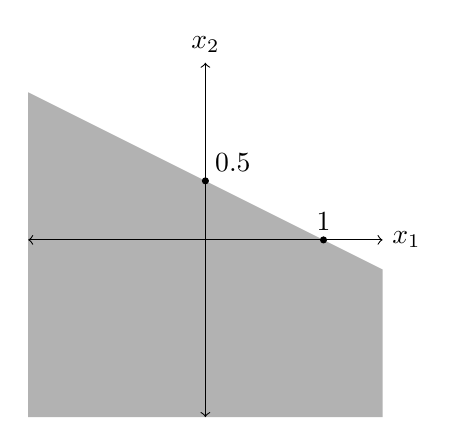
\begin{tikzpicture}[scale=1.5]

					% axes
					\draw [<->] (-1.5,0) -- (1.5,0) node [right] {$x_1$};
					\draw [<->] (0,-1.5) -- (0,1.5) node [above] {$x_2$};

					% set
					\fill [opacity=0.3] (-1.5,-1.5) -- (-1.5,1.25) -- (1.5,-0.25) -- (1.5,-1.5);

					% labels
					\draw [fill] (1,0) circle [radius=0.025]
						node [above] {$1$};
					\draw [fill] (0,0.5) circle [radius=0.025] 
						node [above right] {$0.5$};

				\end{tikzpicture}
			\end{center}
		\end{solution}


		\item
		$B=\{x\in\R^2:x_1^2\le x_2\}$.
		%
		\begin{solution}
			The set~$B$ is convex and is shown below.
			%
			\begin{center}
				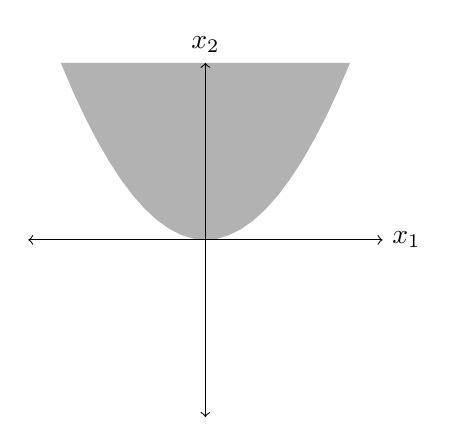
\begin{tikzpicture}[scale=1.5]

					% axes
					\draw [<->] (-1.5,0) -- (1.5,0) node [right] {$x_1$};
					\draw [<->] (0,-1.5) -- (0,1.5) node [above] {$x_2$};

					% set
					\fill [opacity=0.3] [domain=-1.2247:1.2247] plot (\x, {\x*\x});
					
				\end{tikzpicture}
			\end{center}
		\end{solution}

		\item
		$C=\{x\in\R^2:x_1^2\ge x_2\}$.
		%
		\begin{solution}
			The set~$C$ is shown below.
			It is \emph{not} convex because the line segment connecting the points~$x^1,x^2\in C$ contains points that are not in~$C$.
			%
			\begin{center}
				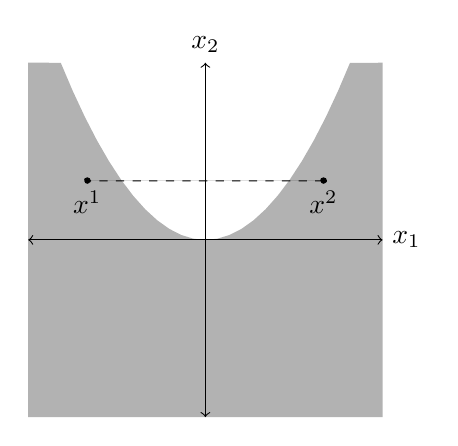
\begin{tikzpicture}[scale=1.5]

					% axes
					\draw [<->] (-1.5,0) -- (1.5,0) node [right] {$x_1$};
					\draw [<->] (0,-1.5) -- (0,1.5) node [above] {$x_2$};

					% set
					\fill [opacity=0.3] [domain=-1.2247:1.2247] (-1.5,-1.5) -- (-1.5,1.5) --  plot (\x, {\x*\x}) -- (1.5,1.5) -- (1.5,-1.5);

					% example points
					\draw [fill, dashed] (1, 0.5) circle [radius=0.025] node [below] {$x^2$} -- (-1,0.5) circle [radius=0.025] node [below] {$x^1$};

				\end{tikzpicture}
			\end{center}
		\end{solution}

		\item
		$D=\{x\in\R^2:x_1x_2\le1\}$.
		%
		\begin{solution}
			The set~$D$ is shown below.
			It is \emph{not} convex because the line segment connecting the points~$x^1,x^2\in D$ contains points that are not in~$D$.
			%
			\begin{center}
				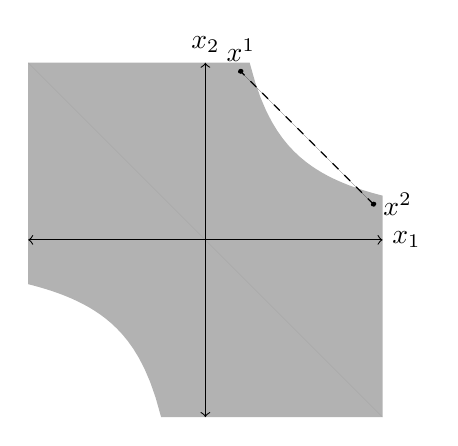
\begin{tikzpicture}[scale=1.125]

					% axes
					\draw [<->] (-2,0) -- (2,0) node [right] {$x_1$};
					\draw [<->] (0,-2) -- (0,2) node [above] {$x_2$};

					% set
					\fill [opacity=0.3] [domain=0.5:2] (-2,2) -- plot (\x, {1/\x}) -- (2,-2);
					\fill [opacity=0.3] [domain=-2:-0.5] (-2,2) -- plot (\x,{1/\x}) -- (2,-2);

					% example points
					\draw [fill, dashed] (1.9,0.4) circle [radius=0.025] node [right] {$x^2$} -- (0.4,1.9) circle [radius=0.025] node [above] {$x^1$};

				\end{tikzpicture}
			\end{center}
		\end{solution}

		\item
		$E=\{x\in\R^2:x_1x_2\ge1\}$.
		%
		\begin{solution}
			The set~$E$ is shown below.
			It is \emph{not} convex because the line segment connecting the points~$x^1,x^2\in E$ contains points that are not in~$E$.
			%
			\begin{center}
				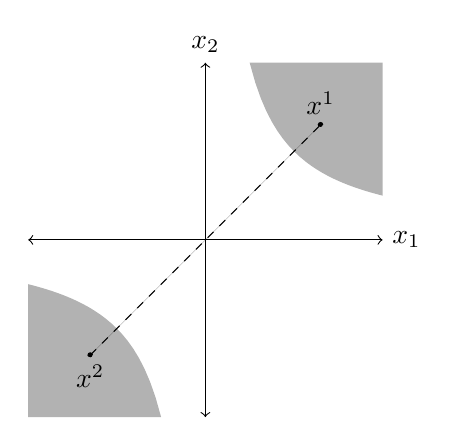
\begin{tikzpicture}[scale=1.125]

					% axes
					\draw [<->] (-2,0) -- (2,0) node [right] {$x_1$};
					\draw [<->] (0,-2) -- (0,2) node [above] {$x_2$};

					% set
					\fill [opacity=0.3] [domain=0.5:2] plot (\x, {1/\x}) -- (2,2);
					\fill [opacity=0.3] [domain=-2:-0.5] plot (\x,{1/\x}) -- (-2,-2);

					% example points
					\draw [fill, dashed] (-1.3,-1.3) circle [radius=0.025] node [below] {$x^2$} -- (1.3,1.3) circle [radius=0.025] node [above] {$x^1$};


				\end{tikzpicture}
			\end{center}
		\end{solution}

	\end{enumerate}

\end{enumerate}
